\chapter{Technical Discussion}
The focus of this technical investigation was to develop my knowledge of the NoSQL and indexing solutions examined in the project and to gain insight into the subject matter by reflecting on previously conducted research. Prior to this research, my understanding of the functionality provided by Neo4j and Apache Cassandra was minimal. Throughout my university degree I have undertaken modules which have stipulated a working knowledge of MySQL as a prerequisite therefore my comprehension of MySQL is proficient. - EXPAND

\section{Database Classification}
One of the first decisions to be made when when selecting a database is the characteristics of the data you are looking to leverage. (Dash, 2013) There are a multitude of options available with many different classifications. - EXPAND

\subsection{Document-Oriented Database}
Document-orientated database (DODB) are designed for storing, retrieving and managing document files such as XML, JSON and BSON. The documents stored in a DODB model are data objects which describe the data in the document, as well as the data itself. - EXPAND

\subsubsection{MongoDB}\label{mongo}
One of the most popular NoSQL technologies is MongoDB. MongoDB is an open source cross-platform DODB. The premise for using MongoDB is simplicity, speed and scalability (MongoDB White Paper, 2015). Its ever growing popularity, specifically amongst programmers, stems from the unrestrictive and flexible DODB data model which gives you the ability to query on all fields and boasts instinctive mapping of objects in modern programming languages. (MongoDB White Paper, 2015) The database design of MongoDB is based on the JSON file format named BSON.

*NOTES* A record in MongoDB is stored in collections. A collection is a grouping of MongoDB documents.
Within this free flowing environment documents can become as sophisticated and complex as required; information about a document record can be sub categorised by the integration of nested data. *NOTES*

EXPAND - FUNCTIONALITY? 

\subsection{Graph-Orientated Database}
A graph-oriented database (GODB), is a form of NoSQL database solution that uses graph theory to store, map and query relationships. A graph is a collection of nodes connected by relationships. "Graphs represent entities as nodes and the ways in which those entities relate to the world as relationships." (Robinson, Webber and Eifrem, 2015) The formation of the graph database structure is extremely useful and eloquent as it permits clear modelling of a vast and often ecliptic array of data types. (Robinson, Webber and Eifrem, 2015) An example of data represented in a graph structure is the Twitter relationship model. \begin{center}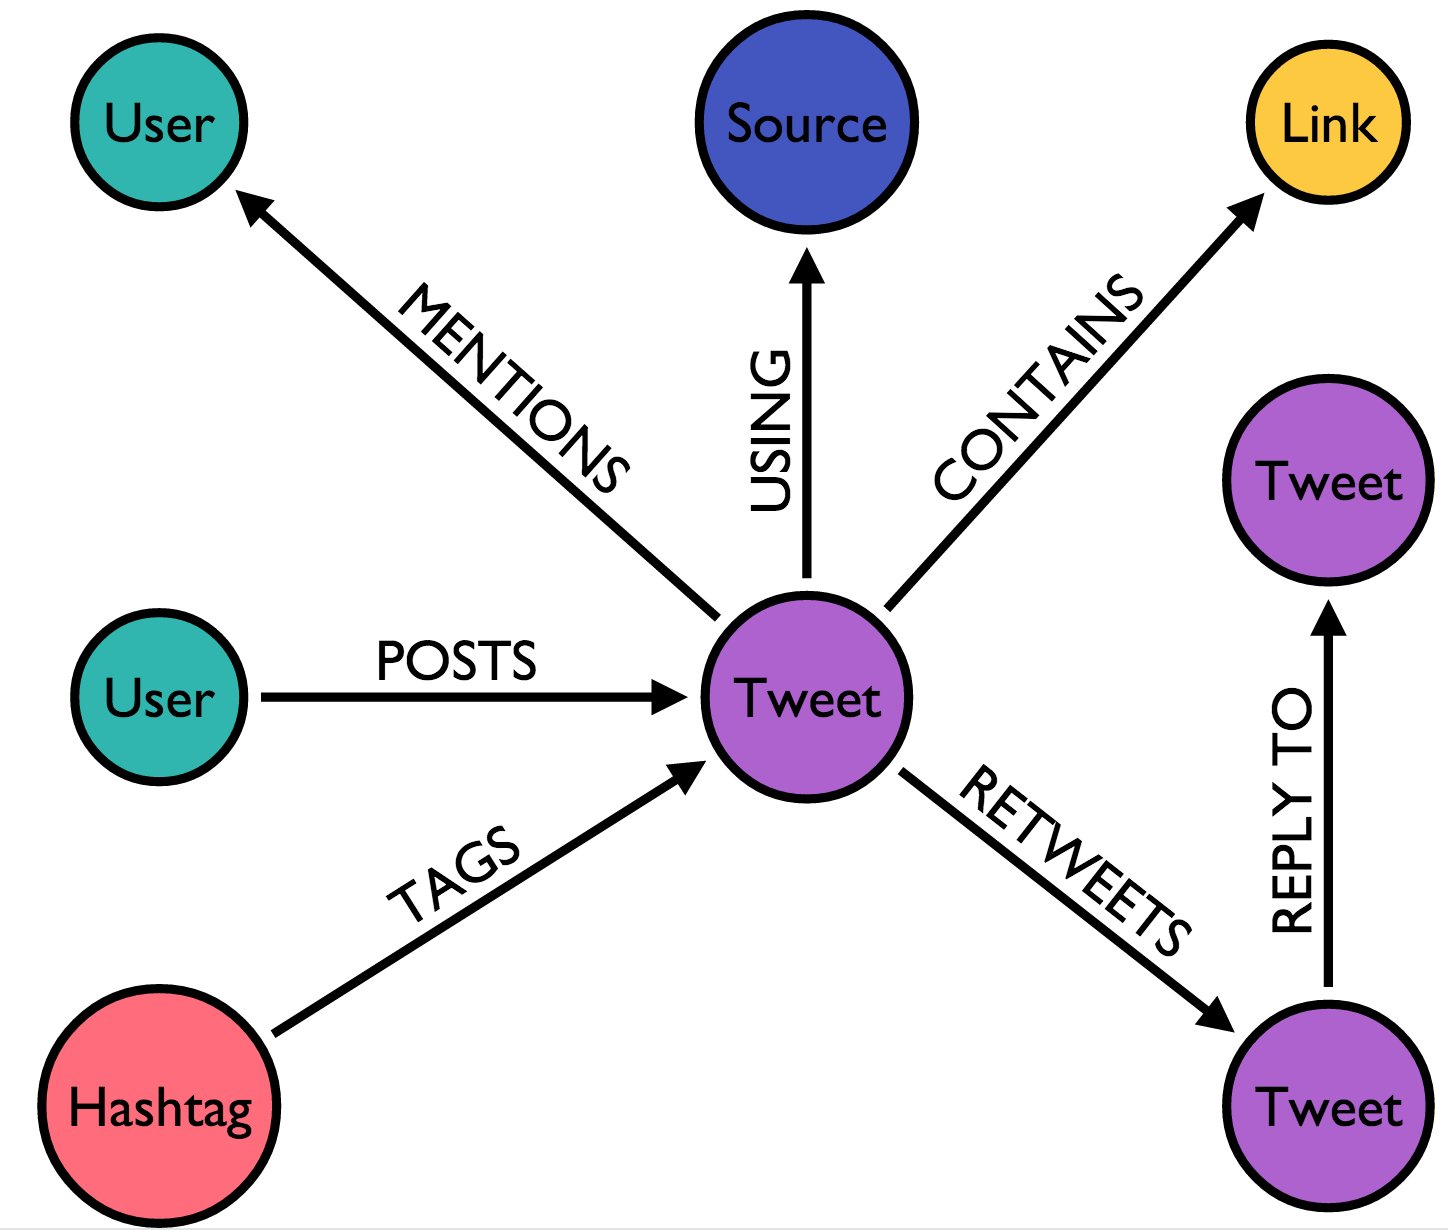
\includegraphics[width=0.3\linewidth]{images/graphdb_twitter}\end{center}  Figure[ADD FIGURE REF] illustrates the nodes involved in a standard tweet and the relationship link between them. The labeled nodes indicate the various operations which are involved in one the tweet. One interpretation of the [FIGURE REF] example is that a user posts a tweet, using the Twitter App which mentions another user and includes a hashtag and link. - REVISE

\subsubsection{Neo4j}\label{neo}
Neo4j is an open-source NoSQL GODB which imposes the Property Graph Model throughout its implementation. The team behind the development of Neo4j describe it as an "An intuitive approach to data problems"(Neo4j web ref). One of the reasons in which Neo4j is favoured predominantly amongst database administrators and developers is its efficiency and high scalability. This is in part due to its compact storage and memory caching for the graphs. "Neo4j scales up and out, supporting tens of billions of nodes and relationships, and hundreds of thousands of ACID transactions per second."(Neo4j web ref) - FINISH WRITNG UP NOTES

EXPAND - FUNCTIONALITY? 

\subsection{Distributed Database}
\begin{wrapfigure}{r}{0.5\textwidth}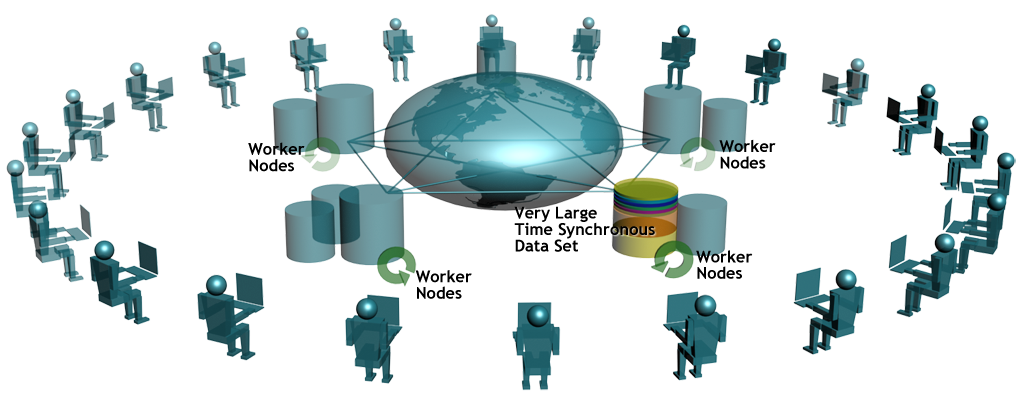
\includegraphics[width=0.9\linewidth]{images/ddelogo}\end{wrapfigure} A distributed database (DDB) comprises of two or more data files located at different sites and servers on a computer network. (DD ref) The advantage of using a DD is that as the database is distributed, multiple users can access a portion of the database at different locations locally and remotely without obstructing one another's work. It is  pivotal for the DD database management system to periodically synchronise the scattered databases to make sure that they all have consistent data. (DD ref) For example if a user updates or deletes data in one location is is essential this change is mirrored on all databases. This ability to remotely access a database from all across the world lends itself to not only multinational companies for example but also startup businesses which recruit the expertise of others from various locations.

\subsubsection{Apache Cassandra}\label{cassandra}
WRITE UP NOTES
\subsection{Relational Database}
A relational database (RDB) is a collection of data items organised as a set of tables, records and columns from which data can be accessed or reassembled in many different ways. (RDB ref) The connected tables are known as relations and contain one or more columns which comprise of data records called rows. Relations can also be instantiated between the data rows to form functional dependencies called keys which are classified as : (RDB ref 2)
\begin{itemize}
\item One to One: One table record relates to another record in another table.
\item One to Many: One table record relates to many records in another table.
\item Many to One: More than one table record relates to another table record.
\item Many to Many: More than one table record relates to more than one record in another table.
\end{itemize} 
\subsubsection{MySQL}\label{mysql}
MySQL is a freely available open source Relational Database Management System (RDBMS) that uses Structured Query Language (SQL). -FINISH WRITING UP NOTES
EXPAND - FUNCTIONALITY? 
\section{Previous Research - Change Heading}
NoSQL has become a bit of a "...ubiquitous and possibly overused term." (Lerman, 2011)
\subsection{TBC}